\section{Evaluasi Model}

Sesuai dengan metrik yang dipaparkan pada Subbab \ref{sec:evaluasi_model}, tahapan evaluasi dilakukan untuk mengukur kemampuan model dalam memprediksi himpunan data uji (\textit{X\_test}) yang belum pernah dipelajari sebelumnya. Kinerja setiap model dianalisis secara komprehensif melalui metrik \textit{Classification Report} guna meninjau pencapaian nilai \textit{Precision}, \textit{Recall}, serta \textit{F1-Score}. Rincian mengenai distribusi hasil prediksi klasifikasi divisualisasikan melalui \textit{Confusion Matrix}. Mengingat tujuan utama dari arsitektur sistem ini adalah untuk mendeteksi penyewa bermasalah (kelas 1), fokus evaluasi difokuskan pada metrik performa terhadap kelas minoritas agar model tidak menghasilkan peringatan keliru (\textit{false alarm}) pada sistem.

\subsection{Analisis Pengaruh Seleksi Fitur}
Sebelum membandingkan performa akhir tiap model secara spesifik, evaluasi dilakukan terhadap efektivitas jumlah fitur yang dilibatkan dalam fase pelatihan. Berdasarkan serangkaian pengujian komparatif, diperoleh kesimpulan analitis sebagai berikut.
\begin{enumerate}
    \item \textbf{Kestabilan Skenario Simulasi vs. Sensitivitas Data Riil}\\ Pada pengujian menggunakan data sintetis sebelumnya, model berbasis pohon keputusan (seperti \textit{Decision Tree}, \textit{Random Forest}, dan \textit{XGBoost}) menunjukkan performa yang sangat stabil dan tidak terpengaruh oleh reduksi dimensi fitur dengan tingkat akurasi konstan di rentang 98,30\% hingga 98,35\%. Namun, pada data riil, karakteristik tersebut memudar akibat variasi informasi yang tidak sebanyak data sintetis. Oleh karena itu, tahapan seleksi fitur—terutama penghapusan atribut statis seperti \texttt{jenis\_sewa} dan \texttt{status\_kewarganegaraan}—menjadi langkah penting guna menghindari beban \textit{noise} yang dapat merusak akurasi komputasi model.
    \item \textbf{Titik Optimal Fitur (\textit{Sweet Spot})}\\ Mengacu pada hasil keluaran seleksi fitur\ref{lamp:A}, penggunaan tiga fitur terpilih (\texttt{lama\_menginap}, \texttt{checkout\_hour}, dan \texttt{checkin\_hour}) terbukti memberikan kinerja yang optimal. Saat dikombinasikan dengan fungsi optimasi pada model misalnya KNN, susunan atribut ini berhasil membuat model berhasil mengidentifikasi 100\% kasus pelanggaran secara absolut pada himpunan data uji (dengan nilai \textit{Recall} 1,0000). Hal ini mengonfirmasi bahwa kombinasi informasi temporal tersebut berguna untuk mendeteksi anomali tanpa membebani pemrosesan atau memicu risiko \textit{overfitting}.
\end{enumerate}

\subsection{Analisis Pengaruh \textit{Hyperparameter Tuning}}
Selain penyesuaian jumlah fitur, proses pencarian parameter optimal (\textit{hyperparameter tuning}) juga memberikan pola yang bervariasi terhadap karakteristik tiap model pada data riil. Berikut adalah penjabaran hasil analisisnya.
\begin{enumerate} 
    
    % \newpage
    \item \textbf{Dampak Positif pada Model Berbasis Jarak}\\ Proses penyesuaian parameter terbukti memberikan peningkatan performa yang signifikan, khususnya pada model \textit{K-Nearest Neighbors} (KNN). Optimasi rentang jarak dan bobot tetangga mampu menaikkan nilai \textit{F1-Score} kelas minoritas dari 0,8649 (versi \textit{default}) menjadi 0,8947 (versi \textit{tuned}). Selain itu, KNN \textit{tuned} sukses mengeliminasi rasio kegagalan deteksi (\textit{False Negative}) sepenuhnya—dari 5,88\% menjadi \textit{Recall} 1,0000—dan hanya menyisakan 4 kasus (\textit{False Positive}). Sementara itu, model SVM RBF sudah mencapai performa maksimal (nilai \textit{Recall} sempurna) sejak konfigurasi \textit{default}-nya dan tidak menunjukkan perubahan performa pasca \textit{tuning}.
    \item \textbf{Dampak Stagnan pada Sebagian Model Berbasis Pohon}\\ Berbanding terbalik dengan kelompok model berbasis jarak, kinerja \textit{Decision Tree} dan \textit{XGBoost} pada data riil tidak memperlihatkan peningkatan performa. Tingkat akurasi pada \textit{Decision Tree} (96,33\%) dan \textit{XGBoost} (96,33\%) tetap stagnan dan sama persis dengan performa konfigurasi model versi \textit{default}. Model berbasis pohon ini tertahan pada angka (\textit{False Positive}) sebanyak 4 kasus. Namun, anomali positif terjadi pada \textit{Random Forest} yang berhasil memperbaiki kinerjanya dari tingkat akurasi 95,41\% (versi \textit{default}) menjadi 96,33\% setelah dilakukan \textit{tuning}.
\end{enumerate}

\subsection{Hasil Akhir Evaluasi dan Pemilihan Model Terbaik}
Kelima model klasifikasi dievaluasi kinerjanya dalam dua skenario utama, yakni pengujian menggunakan model tanpa (\textit{tuning}) dan model dengan penyesuaian parameter tingkat lanjut (\textit{hyperparameter tuning}). Pengujian final ini dieksekusi menggunakan tiga fitur terpilih, yaitu (\texttt{lama\_menginap}, \texttt{checkout\_hour}, dan \texttt{checkin\_hour}). Seluruh hasil pengujian yang mencakup nilai \textit{Precision}, \textit{Recall}, dan \textit{F1-Score} dari masing-masing model—baik untuk deteksi kelas 0 (Normal) maupun kelas 1 (Melanggar) dapat dilihat pada Tabel~\ref{tab:model_comparison}.

\begin{table}[H]
\centering
\caption{Perbandingan Performa Keseluruhan Model pada Data Riil: Tanpa Tuning dan Dengan Tuning}
\label{tab:model_comparison}
\resizebox{\textwidth}{!}{
    \begin{tabular}{|l|l|c|c|c|c|c|c|c|}
    \hline
    \multirow{2}{*}{\textbf{Model}} & \multirow{2}{*}{\textbf{Kondisi}} & \multicolumn{3}{c|}{\textbf{Kelas 0 (Normal)}} & \multicolumn{3}{c|}{\textbf{Kelas 1 (Melanggar)}} & \multirow{2}{*}{\textbf{Akurasi}} \\ \cline{3-8}
    & & \textbf{Precision} & \textbf{Recall} & \textbf{F1-Score} & \textbf{Precision} & \textbf{Recall} & \textbf{F1-Score} & \\
    \hline
    \multirow{2}{*}{Decision Tree} 
    & Tanpa Tuning & 1.0000 & 0.9565 & 0.9778 & 0.8095 & 1.0000 & 0.8947 & 0.9633 \\ \cline{2-9}
    & Dengan Tuning & 1.0000 & 0.9565 & 0.9778 & 0.8095 & 1.0000 & 0.8947 & 0.9633 \\
    \hline
    \multirow{2}{*}{Random Forest} 
    & Tanpa Tuning & 0.9888 & 0.9565 & 0.9724 & 0.8000 & 0.9412 & 0.8649 & 0.9541 \\ \cline{2-9}
    & Dengan Tuning & 1.0000 & 0.9565 & 0.9778 & 0.8095 & 1.0000 & 0.8947 & 0.9633 \\
    \hline
    \multirow{2}{*}{{KNN}} 
    & Tanpa Tuning & 0.9888 & 0.9565 & 0.9724 & 0.8000 & 0.9412 & 0.8649 & 0.9541 \\ \cline{2-9}
    & {Dengan Tuning} & {1.0000} & {0.9565} & {0.9778} & {0.8095} & {1.0000} & {0.8947} & {0.9633} \\
    \hline
    \multirow{2}{*}{SVM (RBF)} 
    & Tanpa Tuning & 1.0000 & 0.9565 & 0.9778 & 0.8095 & 1.0000 & 0.8947 & 0.9633 \\ \cline{2-9}
    & Dengan Tuning & 1.0000 & 0.9565 & 0.9778 & 0.8095 & 1.0000 & 0.8947 & 0.9633 \\
    \hline
    \multirow{2}{*}{XGBoost} 
    & Tanpa Tuning & 1.0000 & 0.9565 & 0.9778 & 0.8095 & 1.0000 & 0.8947 & 0.9633 \\ \cline{2-9}
    & Dengan Tuning & 1.0000 & 0.9565 & 0.9778 & 0.8095 & 1.0000 & 0.8947 & 0.9633 \\
    \hline
    \end{tabular}
}
\end{table}
                         
Berdasarkan Tabel~\ref{tab:model_comparison} menunjukkan bahwa metode \textit{hyperparameter tuning} pada data riil memberikan peningkatan performa pada model \textit{K-Nearest Neighbors} (KNN) dan \textit{Random Forest}. Evaluasi ini memperlihatkan bahwa KNN versi \textit{tuned} sukses mengatasi performa sub-optimal yang dialami oleh model versi \textit{default}. Seluruh model klasifikasi dengan \textit{hyperparameter tuning} pada akhirnya berhasil mencapai titik puncak performa yang seragam dengan tingkat akurasi (\textbf{96,33\%}) menjadikannya setara dengan model lainnya pada versi \textit{tuned}, namun KNN (bersama \textit{Random Forest}) menunjukkan peningkatan performa paling transformatif dibandingkan performa awal tanpa \textit{tuning}. Selain itu, seluruh model \textit{tuned} mampu mereduksi risiko kesalahan klasifikasi terhadap kelas minoritas secara sempurna (\textit{Recall} \textbf{1,0000}) dan tetap mempertahankan presisi di angka 0,8095. Rincian perbedaan distribusi prediksi secara menyeluruh untuk setiap model—baik sebelum maupun sesudah dilakukan optimasi parameter—dapat dilihat melalui visualisasi \textit{Confusion Matrix} berikut.

\begin{figure}[H]
    \centering
    \begin{subfigure}[b]{0.45\textwidth}
        \centering
        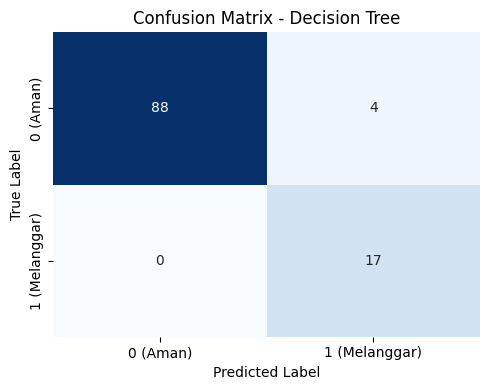
\includegraphics[width=\textwidth]{Gambar/CM_Riil_DT_Tanpa_Tuning.png}
        \caption{Tanpa Tuning}
        \label{fig:cm_dt_tanpa_tuning}
    \end{subfigure}
    \hfill
    \begin{subfigure}[b]{0.45\textwidth}
        \centering
        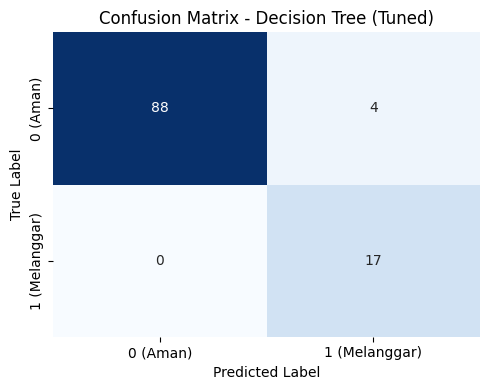
\includegraphics[width=\textwidth]{Gambar/CM_Riil_DT_Tuned.png}
        \caption{Dengan Tuning}
        \label{fig:cm_dt_tuned}
    \end{subfigure}
    \caption{Perbandingan \textit{Confusion Matrix} Model \textit{Decision Tree} (Data Riil)}
    \label{fig:cm_comparison_dt}
\end{figure}

\begin{figure}[H]
    \centering
    \begin{subfigure}[b]{0.45\textwidth}
        \centering
        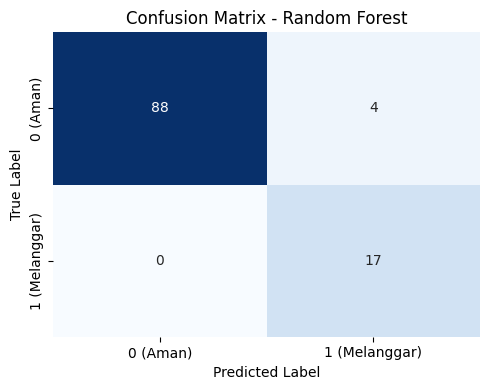
\includegraphics[width=\textwidth]{Gambar/CM_Riil_RF_Tanpa_Tuning.png}
        \caption{Tanpa Tuning}
        \label{fig:cm_rf_tanpa_tuning}
    \end{subfigure}
    \hfill
    \begin{subfigure}[b]{0.45\textwidth}
        \centering
        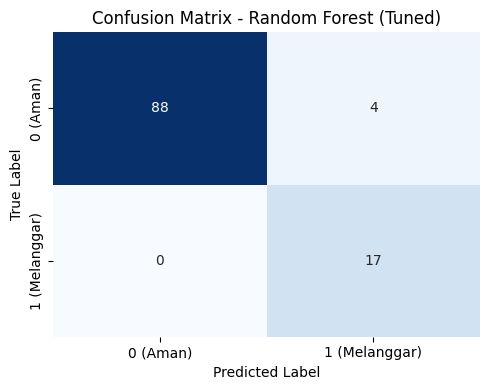
\includegraphics[width=\textwidth]{Gambar/CM_Riil_RF_Tuned.png}
        \caption{Dengan Tuning}
        \label{fig:cm_rf_tuned}
    \end{subfigure}
    \caption{Perbandingan \textit{Confusion Matrix} Model \textit{Random Forest} (Data Riil)}
    \label{fig:cm_comparison_rf}
\end{figure}

\begin{figure}[H]
    \centering
    \begin{subfigure}[b]{0.45\textwidth}
        \centering
        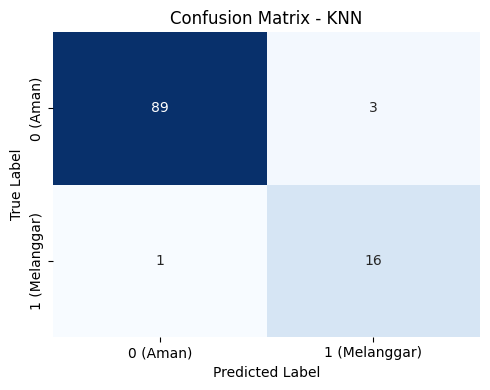
\includegraphics[width=\textwidth]{Gambar/CM_Riil_KNN_Tanpa_Tuning.png}
        \caption{Tanpa Tuning}
        \label{fig:cm_knn_tanpa_tuning}
    \end{subfigure}
    \hfill
    \begin{subfigure}[b]{0.45\textwidth}
        \centering
        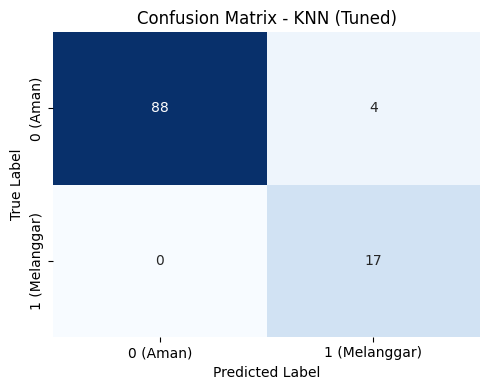
\includegraphics[width=\textwidth]{Gambar/CM_Riil_KNN_Tuned.png}
        \caption{Dengan Tuning}
        \label{fig:cm_knn_tuned}
    \end{subfigure}
    \caption{Perbandingan \textit{Confusion Matrix} Model \textit{K-Nearest Neighbors} / KNN (Data Riil)}
    \label{fig:cm_comparison_knn}
\end{figure}

\begin{figure}[H]
    \centering
    \begin{subfigure}[b]{0.45\textwidth}
        \centering
        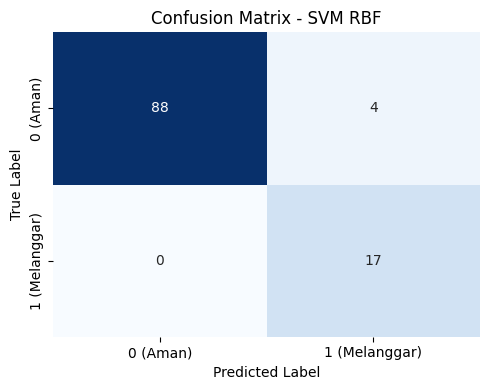
\includegraphics[width=\textwidth]{Gambar/CM_Riil_SVM_Tanpa_Tuning.png}
        \caption{Tanpa Tuning}
        \label{fig:cm_svm_tanpa_tuning}
    \end{subfigure}
    \hfill
    \begin{subfigure}[b]{0.45\textwidth}
        \centering
        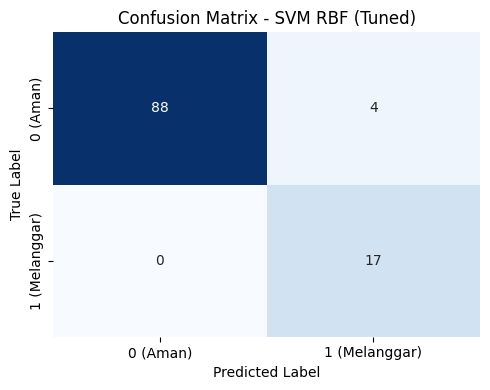
\includegraphics[width=\textwidth]{Gambar/CM_Riil_SVM_Tuned.png}
        \caption{Dengan Tuning}
        \label{fig:cm_svm_tuned}
    \end{subfigure}
    \caption{Perbandingan \textit{Confusion Matrix} Model \textit{Support Vector Machine} / SVM (Data Riil)}
    \label{fig:cm_comparison_svm}
\end{figure}

\begin{figure}[H]
    \centering
    \begin{subfigure}[b]{0.45\textwidth}
        \centering
        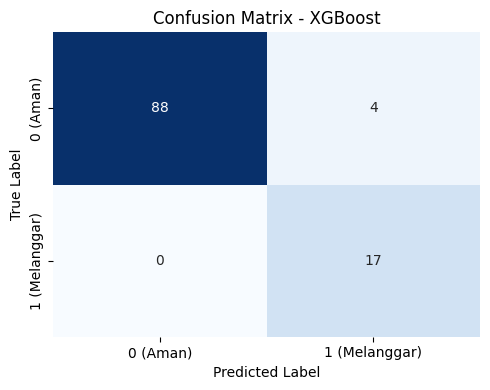
\includegraphics[width=\textwidth]{Gambar/CM_Riil_XGBoost_Tanpa_Tuning.png}
        \caption{Tanpa Tuning}
        \label{fig:cm_xgboost_tanpa_tuning}
    \end{subfigure}
    \hfill
    \begin{subfigure}[b]{0.45\textwidth}
        \centering
        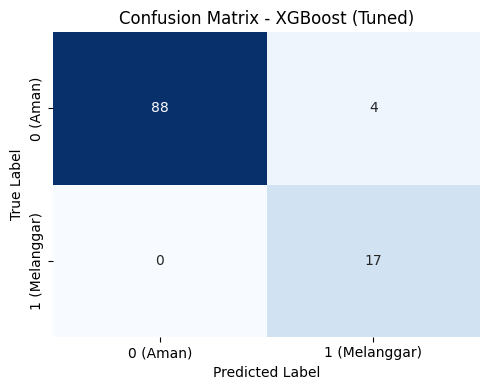
\includegraphics[width=\textwidth]{Gambar/CM_Riil_XGBoost_Tuned.png}
        \caption{Dengan Tuning}
        \label{fig:cm_xgboost_tuned}
    \end{subfigure}
    \caption{Perbandingan \textit{Confusion Matrix} Model \textit{XGBoost} (Data Riil)}
    \label{fig:cm_comparison_xgboost}
\end{figure}

Berdasarkan pemaparan di atas, maka model \textbf{\textit{XGBoost} versi tanpa tuning} ditetapkan secara resmi sebagai arsitektur klasifikasi yang akan diimplementasikan pada sistem. Keputusan ini didasarkan pada pertimbangan bahwa performa versi tanpa {\it tuning} untuk kelompok model berbasis pohon dan jarak tertentu—yakni \textit{XGBoost}, \textit{Decision Tree}, dan SVM—sudah menghasilkan performa yang sangat baik dan optimal dengan tingkat akurasi (\textbf{96,33\%}) serta \textit{Recall} kelas minoritas yang sempurna (\textbf{1,0000}). Di antara ketiga kandidat model optimal tersebut, \textit{XGBoost} dipilih karena memiliki waktu eksekusi prediksi yang paling cepat (Tabel~\ref{tab:waktu_eksekusi}). Berdasarkan hasil pengujian komputasi untuk 1000 iterasi prediksi, \textit{XGBoost} mencatatkan total waktu paling efisien sebesar 3,117823 detik dengan rata-rata waktu per prediksi 0,003118 detik. Durasi komputasi ini lebih cepat dibandingkan dengan \textit{Decision Tree} yang membutuhkan total waktu 3,254093 detik (rata-rata 0,003254 detik) dan SVM yang memerlukan total waktu 3,271034 detik (rata-rata 0,003271 detik). 

\begin{table}[H]
\centering
\caption{Perbandingan Waktu Eksekusi Prediksi Model Tanpa Tuning (1000 Iterasi)}
\label{tab:waktu_eksekusi}
\begin{tabular}{|l|c|c|}
\hline
\textbf{Model} & \textbf{Total Waktu (detik)} & \textbf{Rata-rata Waktu (detik)} \\
\hline
Decision Tree & 3,254093 & 0,003254 \\
\hline
SVM & 3,271034 & 0,003271 \\
\hline
\textbf{XGBoost} & \textbf{3,117823} & \textbf{0,003118} \\
\hline
\end{tabular}
\end{table}
Dengan demikian, konfigurasi \textit{XGBoost} tanpa tuning menjadi opsi terbaik karena mampu memberikan kecepatan pemrosesan tertinggi dalam pendeteksian anomali pelanggaran tata tertib pada sistem.